\chapter{Classification II: Support Vector Machines und KNN}

\section{Support Vector Machines (SVM)}

\begin{mydefinition}
Eine \textbf{SVM} sucht eine Trennlinie (bzw. Trennebene), die zwei Klassen mit möglichst
\textbf{grossem Rand} trennt. Die wichtigsten Punkte nahe an der Grenze heissen
\textbf{Support Vectors}.
\end{mydefinition}

\begin{figure}[H]
    \centering
    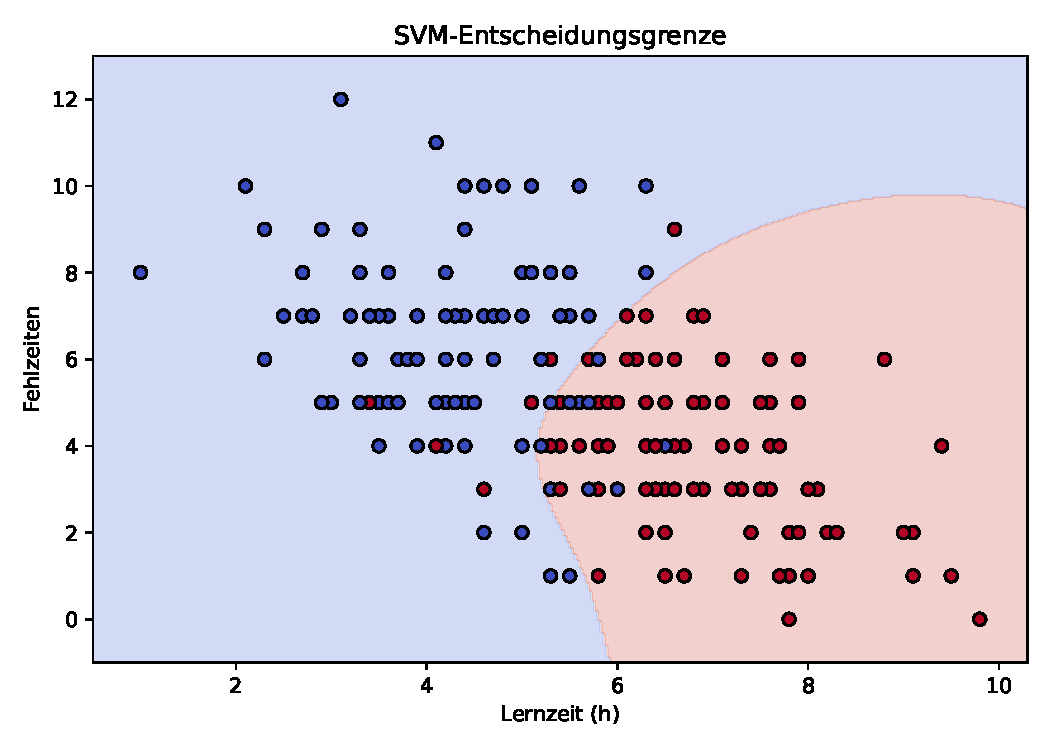
\includegraphics[width=0.72\textwidth]{Grundlagen_Info/15_KI_und_Algorithmen/Figures/svm_boundary.pdf}
    \caption{SVM-Entscheidungsgrenze}
    \label{fig:svm-boundary-15}
\end{figure}

\begin{myexercise}[SVM intuitiv]
Warum kann ein grosser Rand helfen, neue Datenpunkte besser zu klassifizieren?
Erklären Sie mit eigenen Worten in 3--4 Sätzen.
\end{myexercise}

\begin{myremark}[Notebook]
Praktische Umsetzung inkl. Übungen:
\href{\notebookbaseurl03_SVM_Classification.ipynb}{\texttt{03\_SVM\_Classification.ipynb}}
\end{myremark}

\section{k-Nearest Neighbors (KNN)}

\begin{mydefinition}
Beim \textbf{KNN}-Verfahren wird ein neuer Punkt anhand seiner \textbf{k nächsten Nachbarn}
klassifiziert. Die häufigste Klasse in der Nachbarschaft gewinnt.
\end{mydefinition}

\begin{figure}[H]
    \centering
    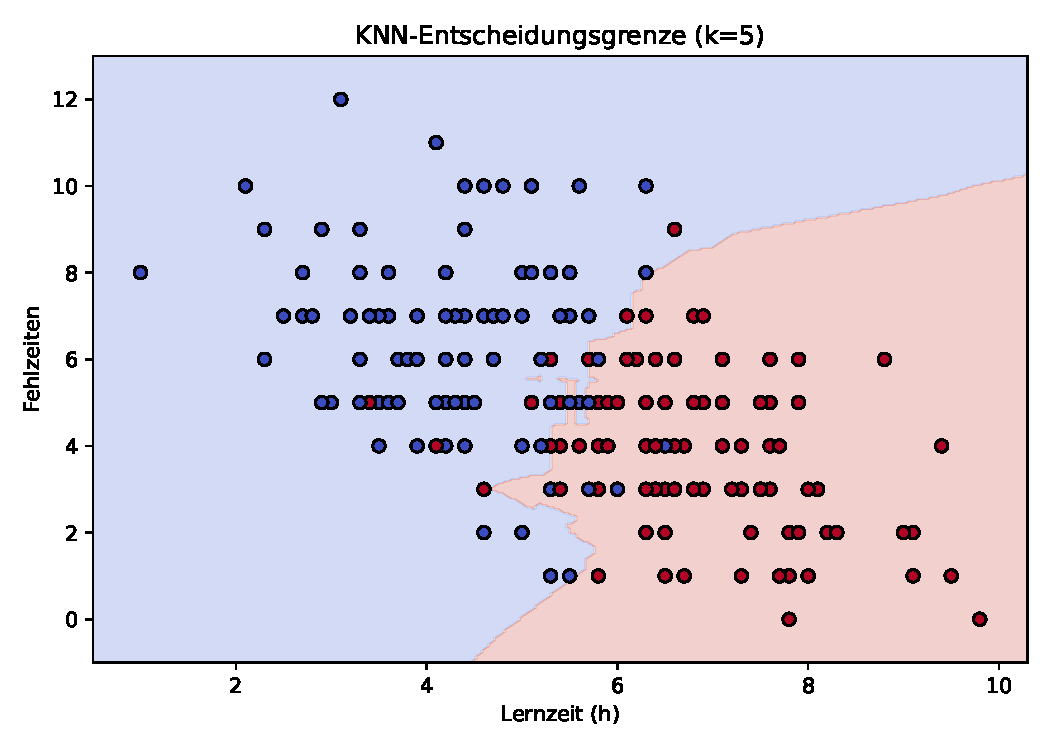
\includegraphics[width=0.72\textwidth]{Grundlagen_Info/15_KI_und_Algorithmen/Figures/knn_boundary.pdf}
    \caption{KNN-Entscheidungsgrenze für ein Beispiel mit zwei Merkmalen}
    \label{fig:knn-boundary-15}
\end{figure}

\begin{myexercise}[Einfluss von \texorpdfstring{$k$}{k}]
Beschreiben Sie den Unterschied zwischen kleinem und grossem \(k\):
\begin{itemize}
    \item Wann reagiert KNN sehr empfindlich auf Ausreisser?
    \item Wann wird die Grenze sehr \enquote{glatt}?
\end{itemize}
\end{myexercise}

\begin{mychallenge}[Parameterwahl]
Testen Sie in einem Notebook \(k=1,3,5,9\) und dokumentieren Sie:
\begin{enumerate}
    \item Trainingsgenauigkeit
    \item Testgenauigkeit
    \item Ihre begründete Wahl für \(k\)
\end{enumerate}
\end{mychallenge}

\begin{myremark}[Notebook]
Praktische Umsetzung inkl. Übungen:
\href{\notebookbaseurl04_KNN_Classification.ipynb}{\texttt{04\_KNN\_Classification.ipynb}}
\end{myremark}
